\chapter{Instruction tuning \& model alignment}

\section{From next token prediction to assistants}

\begin{flushleft}
  \begin{minipage}{0.65\linewidth}
    The LLMs discussed so far are next token predictors.

    ChatGPT-like assistants need to:

    \begin{itemize}
      \item Follow instructions
      \item Provide helpful answers
    \end{itemize}

    HHH objectives:  \textbf{Helpful}, \textbf{Honest}, \textbf{Harmless}


  \end{minipage}%
  \hfill
  \begin{minipage}{0.3\linewidth}
    \centering
    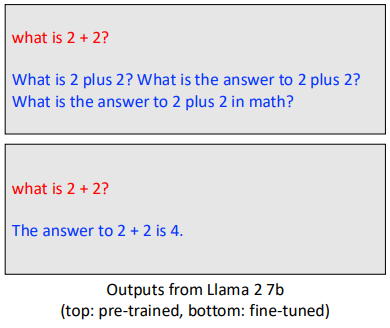
\includegraphics[width=1\linewidth]{content/Parts/images/2026-10-19-11-21-36.png}
  \end{minipage}
\end{flushleft}


\section{Language models are few-shot learners!}

Models have been shown to generalize to new tasks in "fewshot" mode.
Zero-shot performance still low! Explaining the task without
examples was not working well.

We'd like assistants to generalize
without providing new examples
for each task

\section{Including instructions in prompts}
T5 provides a general
architecture that includes
the task to be performed as a
part of the prompt.

The model learns to
condition the answer based
on the request in the input
context.
